\documentclass{beamer}

\usepackage{color}
\usepackage{hyperref}
\usepackage{graphicx}
\usepackage{minted}
\usepackage{bibentry}
\usepackage{import}%
\usepackage{amsmath}%
\usepackage{algorithm}%
\usepackage[noend]{algpseudocode}%
\usepackage{xfrac}
\usepackage{multirow}
\usepackage[utf8x]{inputenc}
\usepackage{bm}%

\usetheme{CambridgeUS}
\usecolortheme{rose}
\setbeamertemplate{navigation symbols}{}%

\AtBeginSection[] {%
  \begin{frame}<beamer>%
    \frametitle{Today's Outline}%
    \tableofcontents[currentsection, subsectionstyle=hide/hide/hide]%
  \end{frame}%
}%

\AtBeginSubsection[]{%
  \begin{frame}<beamer>%
    \frametitle{Today's Outline}%
    \tableofcontents[currentsection, sectionstyle=show/show,
    subsectionstyle=show/shaded/hide]%
  \end{frame}%
}%

\newcommand{\mytitle}[5]{%
  \title[L#1. #3]{\textbf{Artificial Neural Networks} \\
    Lecture #1: #2}%
  \author[Tudor Berariu (UPB)]{Tudor Berariu \\
    \emph{tudor.berariu@gmail.com} \\
    
\includegraphics[width=0.1\textwidth]{graphics/acs.pdf} \\
    {\footnotesize Faculty of Automatic Control and Computers \\
      University Politehnica of Bucharest}}%
  \date[#4]{Lecture : #4 \\ Last Updated: #5}%
}%

\DeclareMathOperator{\sign}{sign}
\DeclareMathOperator{\argmax}{argmax}
\DeclareMathOperator{\argmin}{argmin}

\newcommand{\defterm}[1]{\alert{\textbf{#1}}}
\newcommand{\ml}[0]{\alert{\textbf{ML}}}

\renewcommand{\algorithmicrequire}{\textbf{Input:}}


\mytitle{1}{Introduction}{Introduction to ANN}{7$^{\text{th}}$ of
  October, 2015} {30$^{\text{th}}$ of December, 2015}

\begin{document}

\begin{frame}[plain]
  \titlepage
\end{frame}

\begin{frame}<beamer>%
  \frametitle{Today's Outline}%
  \tableofcontents[,subsectionstyle=hide/hide/hide]%
\end{frame}%

\section{About this Course}
\label{sec:about}

\subsection{What are Artificial Neural Networks?}
\label{sec:what_are_ann}

\begin{frame}
  \frametitle{What are Artificial Neural Networks?}
  \begin{definition}
    \textbf{Artificial Neural Networks} are \visible<2>{machines
      designed to model the information processing capabilities of
      animal nervous systems.}
  \end{definition}
  \pause
  \vspace*{2em}
  What \emph{information processing capabilities} of the CNS are we
  interested in?
\end{frame}

\begin{frame}
  \frametitle{What do we know about the brain?}
  \begin{itemize}
  \item \textbf{The brain} (nervous system) has a totally
    different architecture from the conventional computer.
  \item \textbf{The brain} is a highly complex, nonlinear, and
    parallel computer (information-processing system). \cite[page
    1]{haykin2009neural}
  \end{itemize}
\end{frame}

\begin{frame}
  \frametitle{What are artificial neural networks?}
  ... back to the definition
  \begin{definition}
    An \textbf{artificial neural network} is a \pause
    \alert<2>{massively parallel distributed} processor \pause made up
    of \alert<3>{simple} processing units \pause that has a natural
    propensity for storing \alert<4>{experiential knowledge} and
    making it available for use.\pause\\It resembles the brain in two
    respects:
    \begin{enumerate}
    \item Knowledge is acquired by the network from its environment
      through a \alert<5>{learning} process.\pause
    \item Interneuron connection strengths, known as synaptic weights,
      are used to store the acquired knowledge.
    \end{enumerate}
    \cite[page 2]{haykin2009neural}
  \end{definition}
\end{frame}

\begin{frame}
  \frametitle{Artificial Neural Networks Description}%
  An ANN consists of a large number of connected computing units:
  \begin{itemize}
  \item input units (correspond to sensory neurons)
  \item hidden units
  \item output units (correspond to motor neurons)
  \end{itemize}
\end{frame}

\begin{frame}
  \frametitle{An example}
  \begin{figure}[h!]
    \centering
    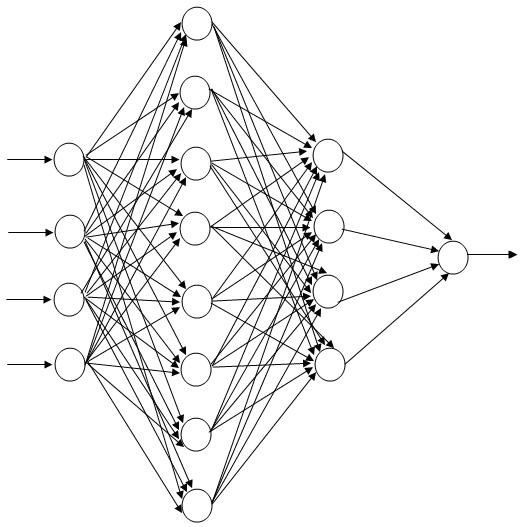
\includegraphics[width=.5\textwidth]{graphics/mlp.jpg}
    \caption{Multi-Layer Feedforward Network}
  \end{figure}
\end{frame}

\begin{frame}
  \frametitle{What are ANNs composed of}%
  The three elements important in any model of ANN:
  \begin{enumerate}
  \item the functions of the nodes
  \item the topology of the network
  \item the learning algorithm
  \end{enumerate}
\end{frame}

\subsection{Why study Artificial Neural Networks?}
\label{sec:why_study}

\begin{frame}
  \frametitle{Why study on ANN begun?}  \textbf{The brain} is many
  times \textbf{faster than} any \textbf{computer} on some specific
  tasks (although its synapses are slow compared to electronic logic
  gates):
  \begin{itemize}
  \item natural language processing
  \item sensorial perception
  \item motor control and movement planning
  \end{itemize}
\end{frame}

\begin{frame}
  \frametitle{What else do we like about the human brain?}  Appealing
  features of the brain:
  \begin{itemize}
  \item adaptivity (learning capabilities)
  \item robustness and fault tolerance
  \item its capability of dealing with fuzzy, noisy, and even
    inconsistent information
  \end{itemize}
\end{frame}

\begin{frame}
  \frametitle{``Single learning algorithm'' hypothesis}
  \begin{figure}[h]
    \centering
    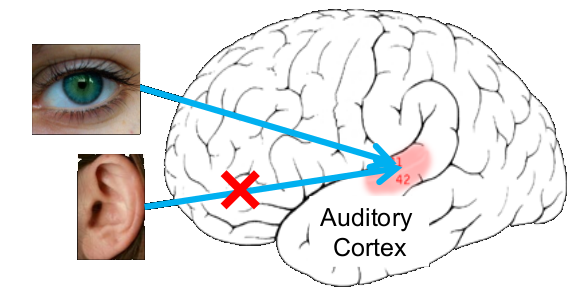
\includegraphics[width=.7\textwidth]{graphics/rewiring.png}
    \caption{Rewiring in ferrets \cite{roe1992visual}}
    \label{fig:rewire}
  \end{figure}
\end{frame}

\begin{frame}
  \frametitle{``Single learning algorithm'' hypothesis}
  \begin{center}
    A blind guy climbing a wall?
  \end{center}
  \begin{center}
    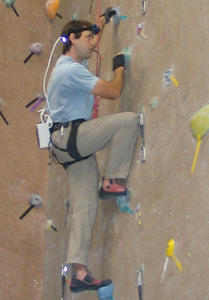
\includegraphics[width=.35\textwidth]{graphics/catarare.jpg}
  \end{center}
\end{frame}

\begin{frame}
  \frametitle{``Single learning algorithm'' hypothesis}
  \begin{center}
    He sees with his tongue...
  \end{center}
  \begin{center}
    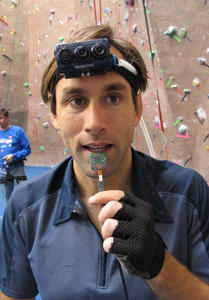
\includegraphics[width=.3\textwidth]{graphics/blind.jpg}
  \end{center}
  \begin{center}
    {\tiny source: \url{http://www.bbc.com/news/health-13358608}}
  \end{center}
\end{frame}

\begin{frame}
  \frametitle{``Single learning algorithm'' hypothesis}
  \begin{center}
    
\includegraphics[width=.5\textwidth]{graphics/third_eye_2.png}%
    \\ \vspace*{1em}
    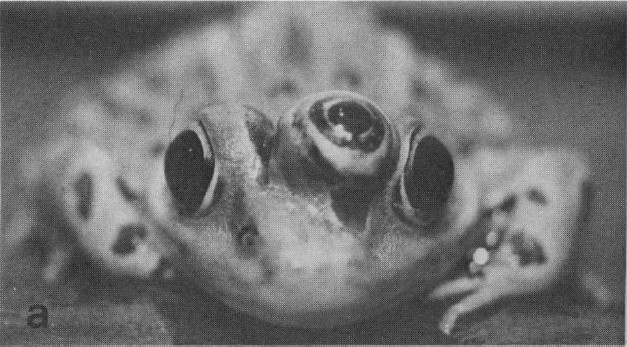
\includegraphics[width=.45\textwidth]{graphics/third_eye.png}%
  \end{center}
  \begin{center}
    \emph{Median third eye was found to develop from transplanted pineal gland} \cite{jangir2005third}
  \end{center}
\end{frame}

% \begin{frame}
%   \frametitle{Successful applications}
%   \begin{itemize}
%   \item stock market prediction \newline \emph{MJ Futures, a company
%       in the stock market industry have made claims that in 2 years
%       they have over 199\% returns based on their predictions made
%       using neural networks.}\\ {\scriptsize
%       (\url{http://cs.stanford.edu/people/eroberts/courses/soco/projects/neural-networks/Applications/})}
%   \end{itemize}
% \end{frame}

\begin{frame}
  \frametitle{Applications: Automatic Translation in Images}
  \begin{center}
    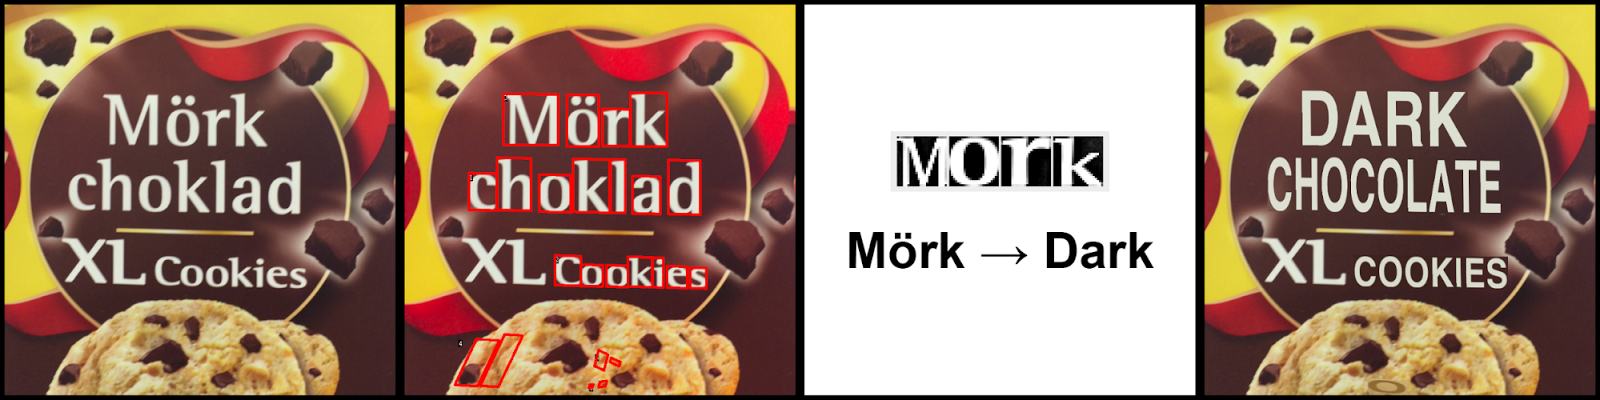
\includegraphics[width=.8\textwidth]{graphics/dark_chocolate}
  \end{center}
  \begin{center}
    {\tiny (source:
      \url{http://googleresearch.blogspot.ro/2015/07/how-google-translate-squeezes-deep.html})}
  \end{center}

\end{frame}

\begin{frame}
  \frametitle{Applications: Speech Recognition}
  \begin{center}
    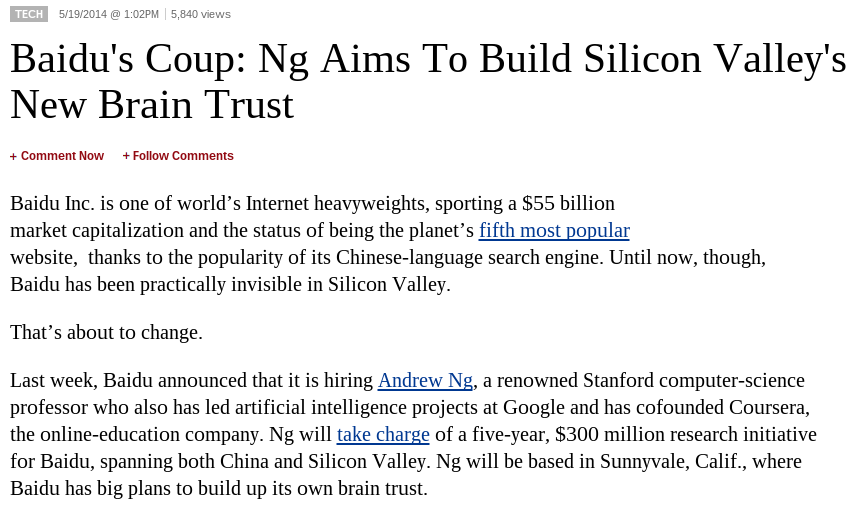
\includegraphics[width=.8\textwidth]{graphics/baidu1}
  \end{center}
  \begin{center}
    {\tiny (source: \url{http://www.forbes.com/sites/georgeanders/2014/05/19/baidus-coup-ng-aims-to-build-silicon-valleys-new-brain-trust/})}
  \end{center}
\end{frame}

\begin{frame}
  \frametitle{Applications: Speech Recognition}
  \begin{itemize}
  \item Baidu used RNN to build a speech recognition system:
    DeepSpeech
  \end{itemize}
  \begin{center}
    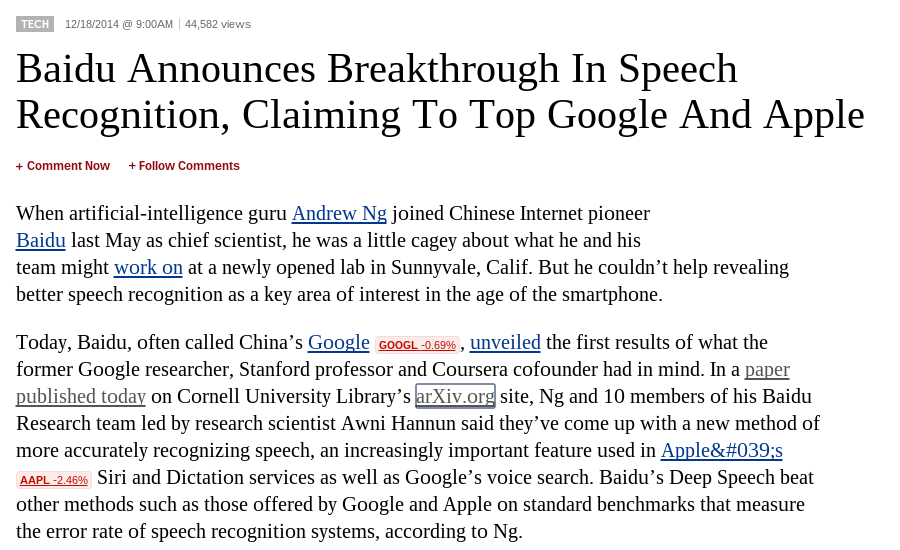
\includegraphics[width=.5\textwidth]{graphics/baidu}
  \end{center}
  \begin{center}{\small
    \nobibliography* \bibentry{hannun2014deepspeech}
  }\end{center}
  \begin{center}
    {\tiny (source:
      \url{https://gigaom.com/2014/12/18/baidu-claims-deep-learning-breakthrough-with-deep-speech/})}
  \end{center}

\end{frame}

\begin{frame}
  \frametitle{Applications: Face detection}
  \begin{figure}[h!]
    \centering
    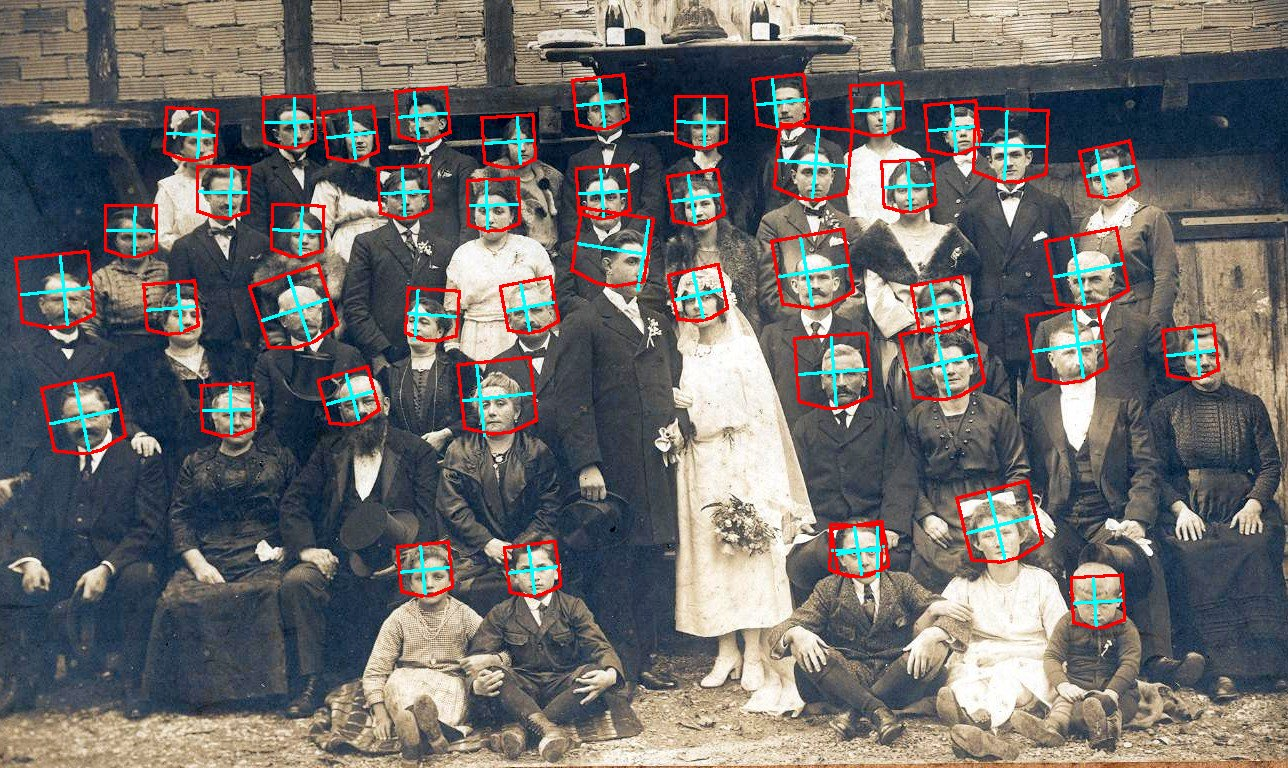
\includegraphics[width=.8\textwidth]{graphics/facetest-alric.jpg}
    \caption{Face detection {\tiny (source:
        \url{http://www.cs.nyu.edu/~yanqn/research/cface/})}}
    \label{fig:lecunface}
  \end{figure}
\end{frame}

\begin{frame}
  \frametitle{Applications: Object Recognition}
  \begin{figure}[h!]
    \centering
    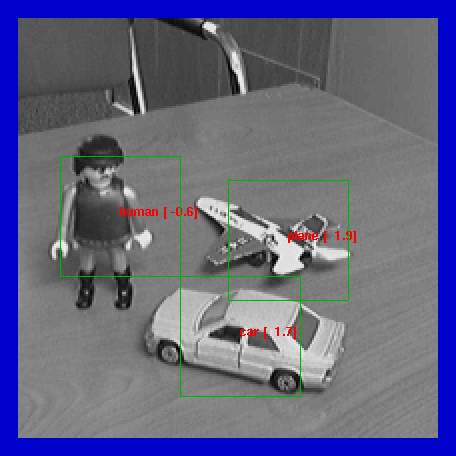
\includegraphics[height=.6\textheight]{graphics/norb.png}
    \caption{Object detection and recognition {\tiny (source:
        \url{http://www.cs.nyu.edu/~yann/research/norb/})}}
    \label{fig:lecunface}
  \end{figure}
\end{frame}

\begin{frame}
  \frametitle{GoogLeNet @ ILSVRC 2014}
  \begin{figure}[h!]
    \centering
    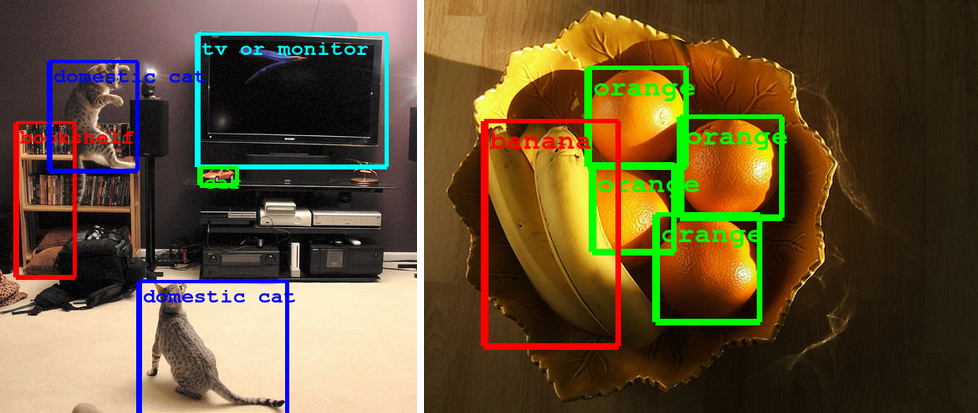
\includegraphics[height=.45\textheight]{graphics/googlenet.png}
    \label{fig:googlenet}
  \end{figure}

  \begin{itemize}
  \item 6.7\% error rate for Hit@5 classification test
  \item {\tiny
      \url{http://karpathy.github.io/2014/09/02/what-i-learned-from-competing-against-a-convnet-on-imagenet/}}
  \item {\tiny
      \url{http://googleresearch.blogspot.ro/2014/09/building-deeper-understanding-of-images.html}}
  \end{itemize}
\end{frame}

\subsection{Course Syllabus}
\label{sec:syllabus}

\begin{frame}[t]
  \frametitle{Course syllabus}%
  \begin{columns}%
    \column{.45\textwidth}%
    \begin{itemize}%
    \item<1-> \alert<1>{ADALINE and the Perceptron}%
    \item<2-> \alert<2>{Multi-Layer Feedforward Networks}%
    \item<3-> \alert<3>{Convolutional Neural Networks}%
    \item<4-> \alert<4>{Hopfield Networks}%
    \item<5-> \alert<5>{Boltzmann Machines}%
    \item<6-> \alert<6>{Autoencoders}%
    \item<7-> \alert<7>{Self-Organizing Maps}%
    \item<8-> \alert<8>{Recurrent Networks}%
    \item<9-> \alert<9>{Memory Networks}%
    \end{itemize}%
    \column{.55\textwidth}%
    \only<1>{%
      \centering%
      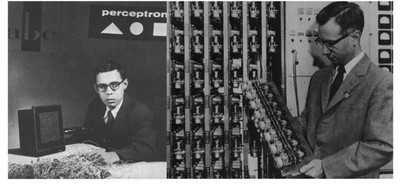
\includegraphics[width=.7\textwidth]{graphics/rosenblatt.jpg}%
    }%
    \only<2>{%
      \centering%
      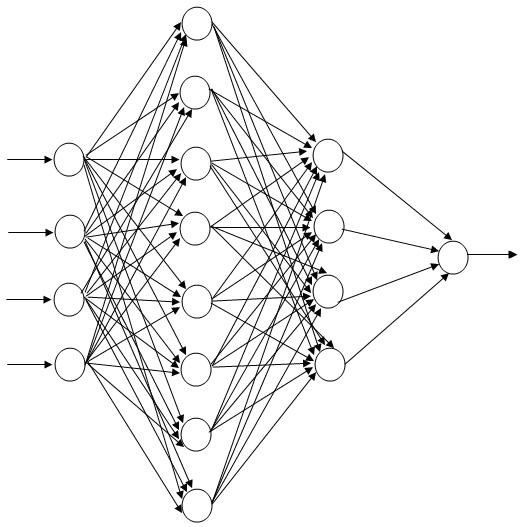
\includegraphics[width=.7\textwidth]{graphics/mlp.jpg}%
    }%
    \only<3>{%
      \centering%
      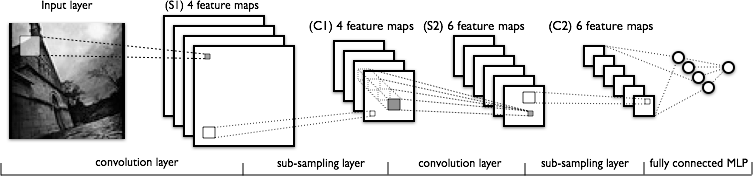
\includegraphics[width=\textwidth]{graphics/mylenet.png}%
      \\
      {\tiny (source: \url{http://deeplearning.net/tutorial/lenet.html})}
    }%
    \only<4>{%
      \centering%
      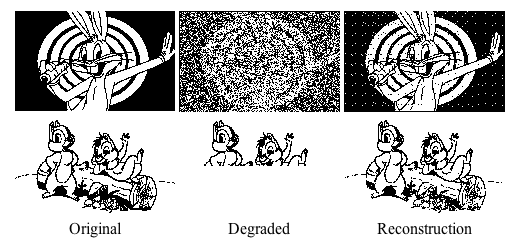
\includegraphics[width=\textwidth]{graphics/hopfieldexample.png}%
      \\
      {\tiny (source: \url{fourier.eng.hmc.edu/e161/lectures/nn/node5.html})}
    }%
    \only<5>{%
      \centering%
      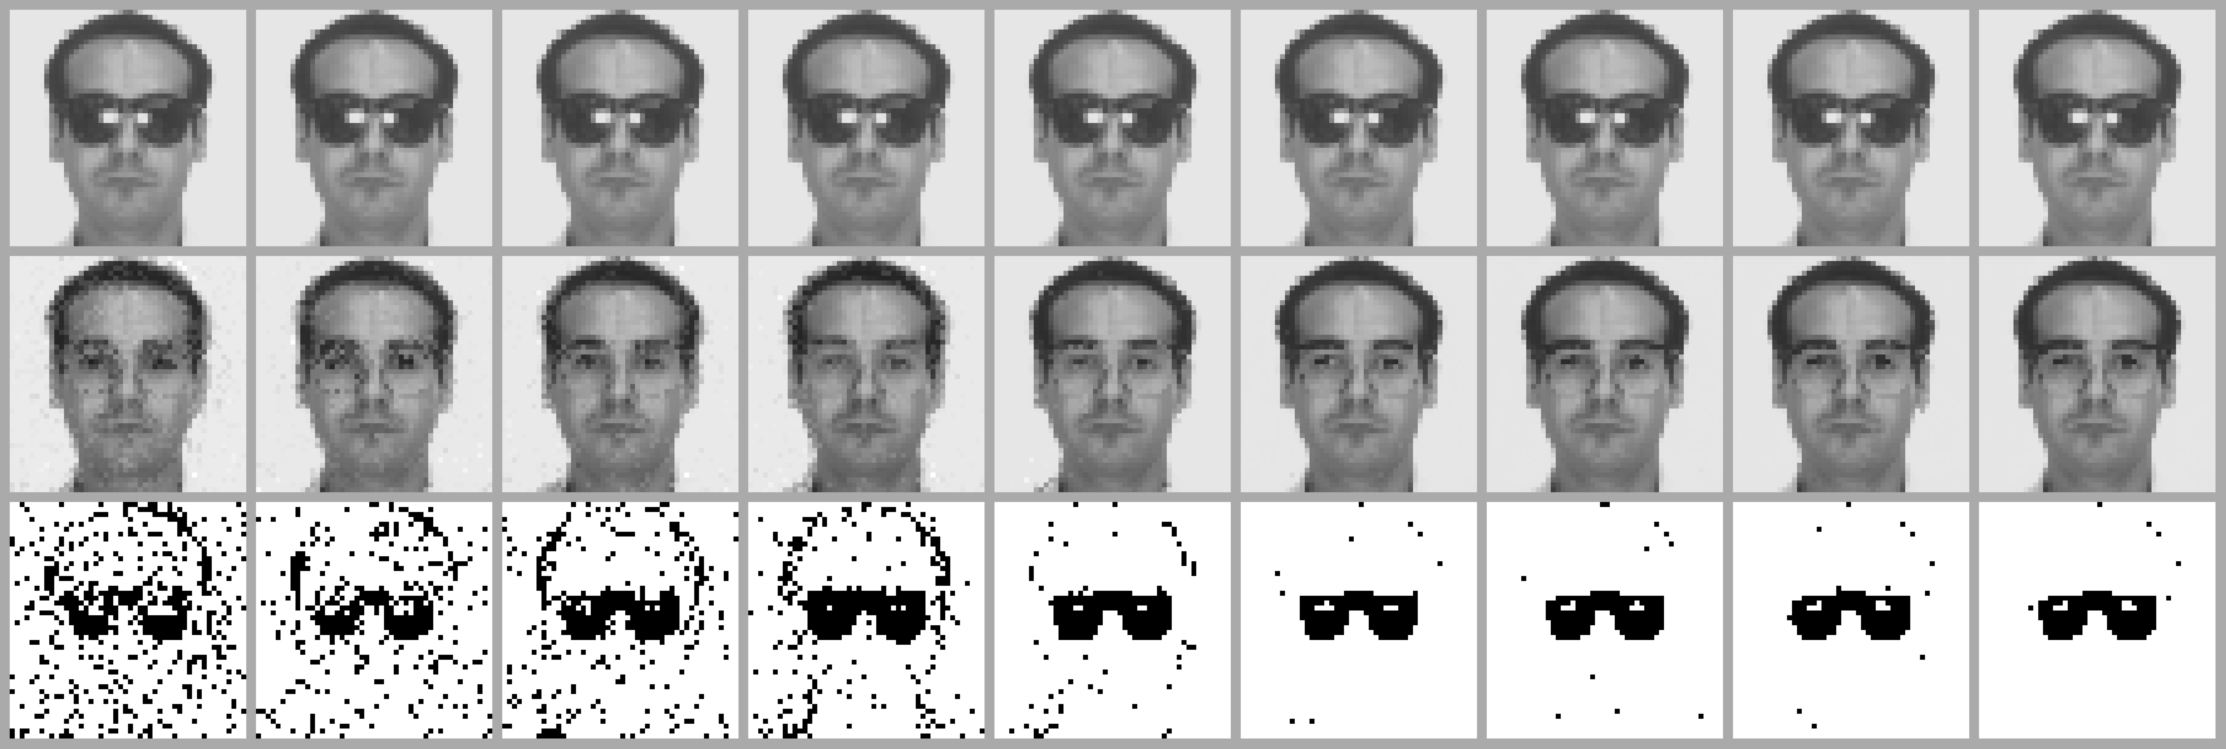
\includegraphics[width=\textwidth]{graphics/robm.png}%
      \\
      (image from \cite{tang2012robust})
    }%
    \only<6>{%
      \centering%
      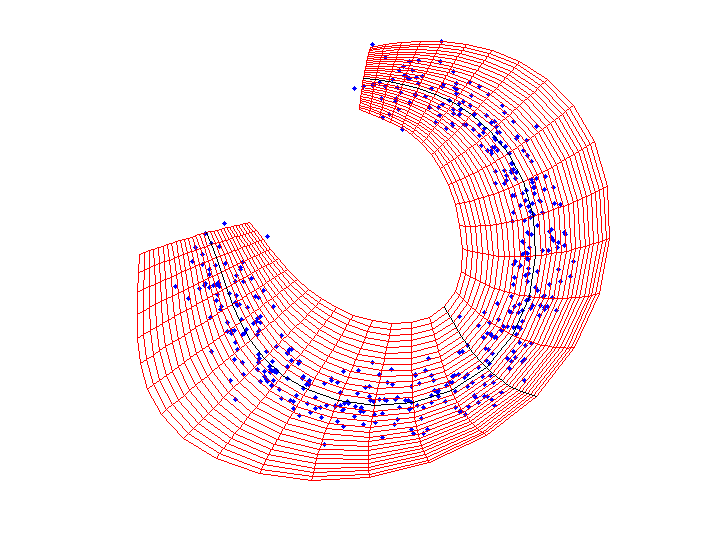
\includegraphics[width=.6\textwidth]{graphics/nlpca.png}%
      \\
      {\tiny (source: \url{http://www.nlpca.org/})}
    }%
    \only<7>{%
      \centering%
      
\includegraphics[width=.9\textwidth]{graphics/maxresdefault.jpg}%
      \\
      {\tiny (source: \url{https://www.youtube.com/watch?v=71wmOT4lHWc})}
    }%
    \only<8>{%
      \centering%
      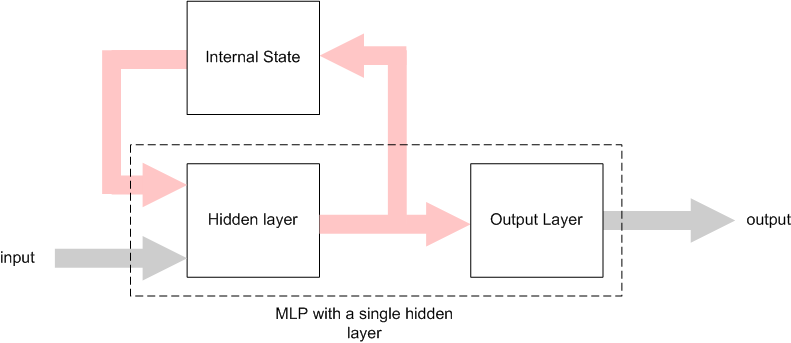
\includegraphics[width=\textwidth]{graphics/elman.png}%
    }%
    \only<9>{%
      \centering%
      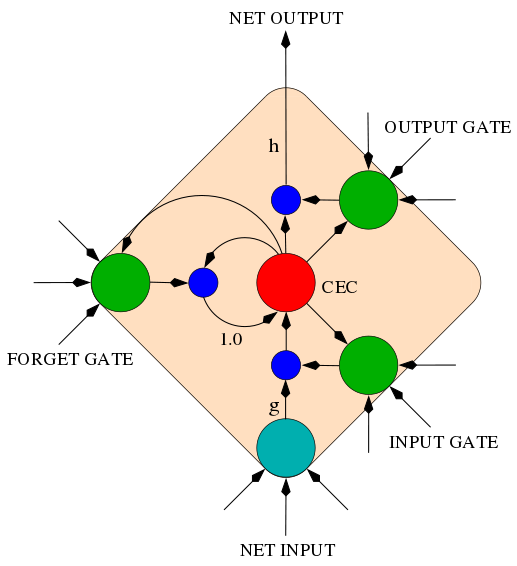
\includegraphics[width=.5\textwidth]{graphics/lstm.png}%
      \\
      {\tiny (source: \url{http://people.idsia.ch/~juergen/rnn.html})}
    }%
    \vfill
    \begin{itemize}%
      \only<1>{%
      \item Both are Single Layer Networks%
      \item Algorithms:%
        \begin{itemize}%
        \item Least Mean Squares Rule (Widrow, Hoff, 1960)%
        \item Perceptron learning (Rosenblatt, 1956)%
        \end{itemize}%
      \item Both solve only linearly separable problems%
      }%
      \only<2>{%
      \item Error Backpropagation%
      \item Learning Algorithms%
      }%
      \only<3>{%
      \item CNNs are used for computer vision problems%
      \item Recently CNNs improved record scores in image recognition
        contests%
      \item CNNs use receptive fields, weight sharing%
      }%
      \only<4>{%
      \item Used for pattern recognition
      \item Auto-associative memories }%
      \only<5>{%
      \item Stochastic version of the Hopfield Network with hidden
        units
      \item Boltzmann Machines escape local minima where Hopfield
        Networks get stuck}%
      \only<6>{%
      \item PCA - finding an lower-dimensional space in which the data
        has the most variance%
      \item PCA with (deep) neural networks%
      }%
      \only<7>{%
      \item Kohonen, 1982%
      \item Extract structure from data (Unsupervised learning
        method)%
      \item Competitive learning%
      }%
      \only<8>{%
      \item feedback loops
      \item internal states
      \item good for sequential data (time series, signal processing)
      \item hard to train }%
      \only<9>{%
      \item LSTM cells \cite{hochreiter1997long}
      \item Neural Turing Machines \cite{graves2014neural}
      \item Memory Networks \cite{weston2014memory} }%
    \end{itemize}
  \end{columns}
\end{frame}

\subsection{Course Goals}
\label{sec:goals}

\begin{frame}
  \frametitle{Course Goals}
  \begin{itemize}
  \item understand the \textbf{fundamental principles} of artificial neural
    networks and their relation to biological systems
  \item understand the \textbf{different architectures} of neural networks
  \item learn how to \textbf{train} neural networks
  \item know which \textbf{problems} are suitable for neural networks
  \item familiarize yourself with \textbf{Torch}
  \end{itemize}
\end{frame}

\subsection{Resources}
\label{sec:resources}

\begin{frame}
  \nobibliography*
  \frametitle{Haykin, 2009}%
  \begin{columns}%
    \column{.35\textwidth}%
    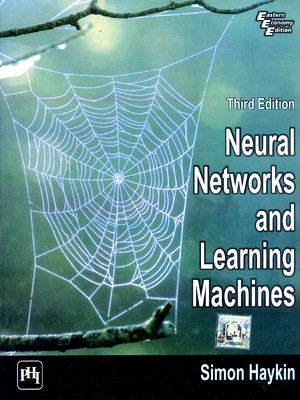
\includegraphics[width=\textwidth]{graphics/book_haykin.jpeg}%
    \column{.55\textwidth}%
    \bibentry{haykin2009neural}%
  \end{columns}%
\end{frame}

\begin{frame}
  \frametitle{Bishop, 1995}%
  \begin{columns}%
    \column{.35\textwidth}%
    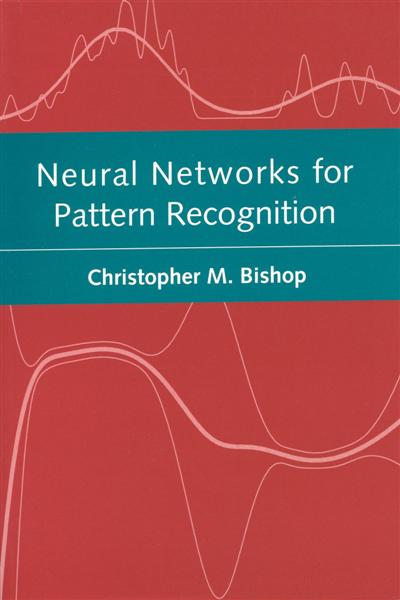
\includegraphics[width=\textwidth]{graphics/book_bishop.jpg}%
    \column{.55\textwidth}%
    \bibentry{bishop1995neural}%
  \end{columns}%
\end{frame}

\begin{frame}
  \frametitle{More recent resources for deep learning}%
  \begin{center}
    \bibentry{Goodfellow-et-al-2015-Book}
  \end{center}
  \vspace*{1em}
  \begin{center}
    \url{http://www.deeplearningbook.org/}
  \end{center}
  \vfill
  ... plus various recent papers
\end{frame}

\section{Neural Networks for Machine Learning}
\label{sec:ann_ml}

\subsection{Machine Learning Refresher}
\label{sec:refresher}

\begin{frame}
  \frametitle{What is Machine Learning?}
  \begin{definition}
    \alert{Machine Learning} \pause is the field of study that gives
    computers the ability to learn without being explicitly
    programmed. (Arthur Samuel, 1959)
  \end{definition}
\end{frame}

\begin{frame}[t]
  \frametitle{Applications of Machine Learning}
  \begin{itemize}
  \item \alert<1>{Self-Driving Car: Google Car}
  \item \alert<2>{Machine Translation: Google Translate}
  \item \alert<3->{Recommender Systems}
    \begin{itemize}
    \item \alert<3>{Movies: ImDB, NetFlix}
    \item \alert<4>{Intelligent Advertising: Google Ads, Facebook Ads}
    \end{itemize}
  \end{itemize}
  \begin{center}%
    \only<1>{%
      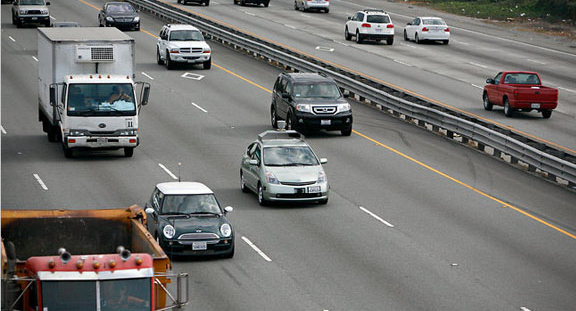
\includegraphics[width=0.45\textwidth]{graphics/google-car-2}%
      \hspace*{2em}%
      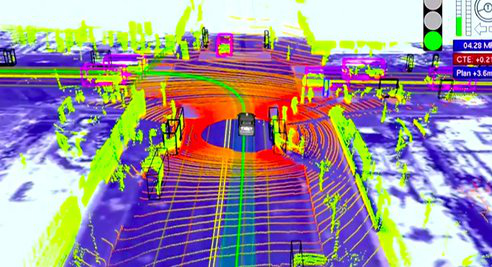
\includegraphics[width=0.45\textwidth]{graphics/google-car}%
      \newline%
      {\scriptsize images from \url{www.nytimes.com}}
    }%
    \only<2>{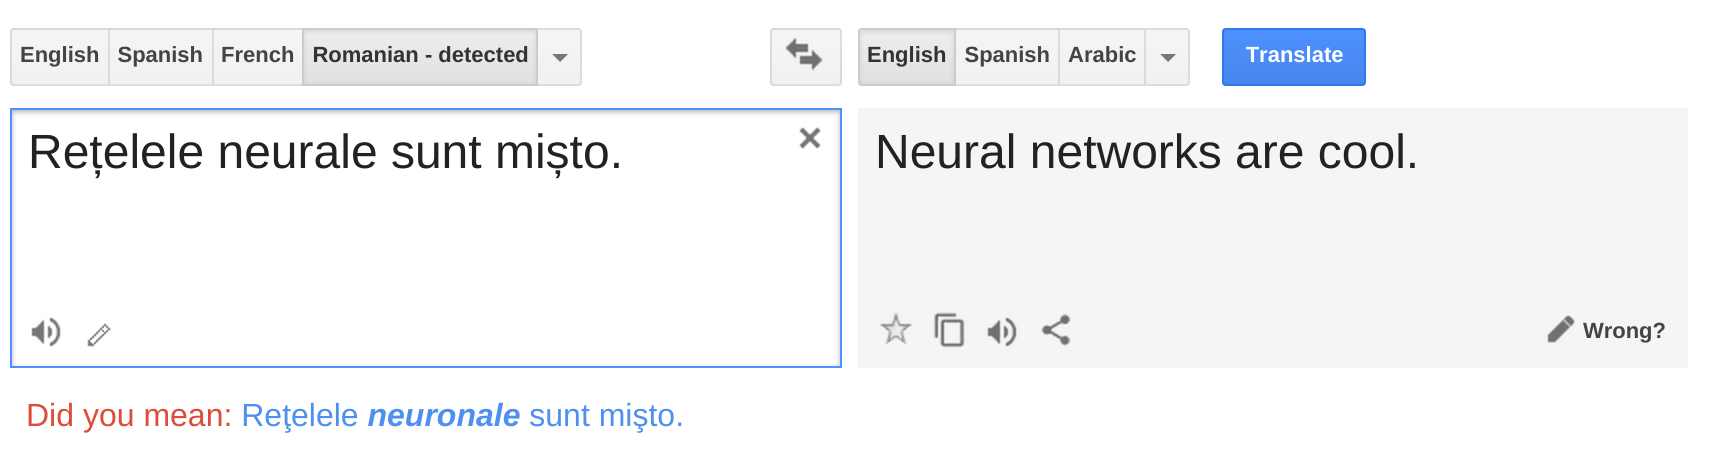
\includegraphics[width=0.9\textwidth]{graphics/translate}}%
    \only<3>{
\includegraphics[width=0.6\textwidth]{graphics/recommender}}%
    \only<4>{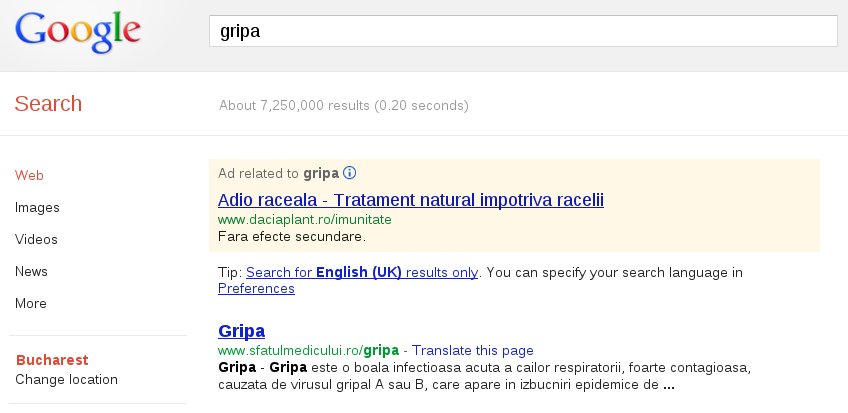
\includegraphics[width=0.65\textwidth]{graphics/gripa}}%
  \end{center}
\end{frame}


\begin{frame}[t]
  \frametitle{Machine Learning: Types of Problems}
  \begin{block}{Problem Types}
    \begin{itemize}
    \item Regression
      \begin{itemize}
      \item predicting the market price of a good
      \end{itemize}%
      \item Classification
        \begin{itemize}
        \item object classification in an image
        \end{itemize}
    \end{itemize}
  \end{block}%
  \begin{center}
    \only<1>{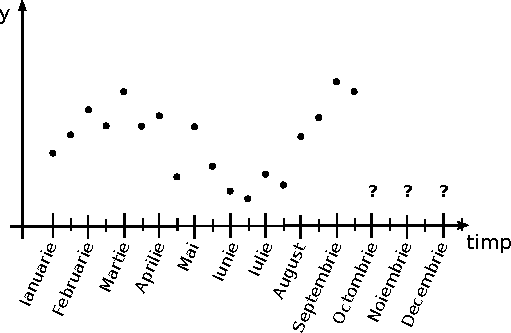
\includegraphics[width=.5\textwidth]{graphics/ml-1}}%
    \only<2>{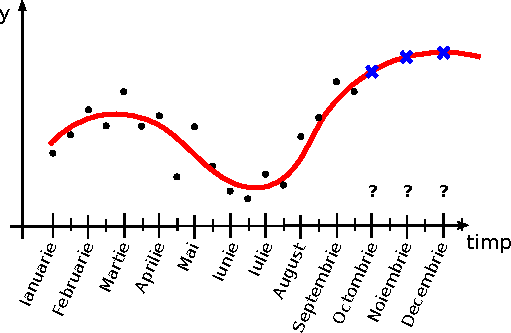
\includegraphics[width=.5\textwidth]{graphics/ml-2}}%
    \only<3>{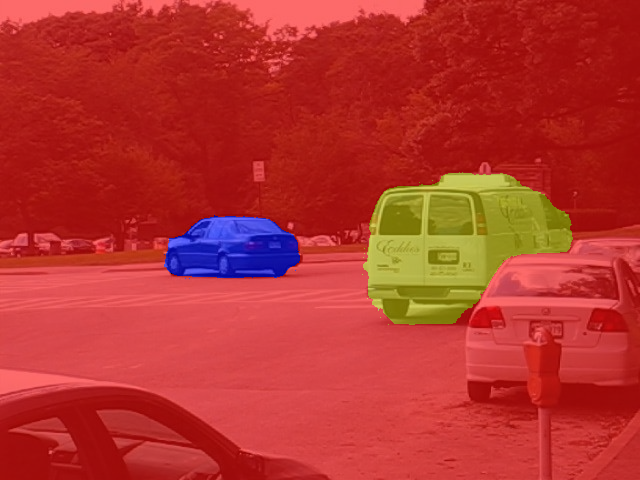
\includegraphics[width=.38\textwidth]{graphics/car-2}}%
    \only<4>{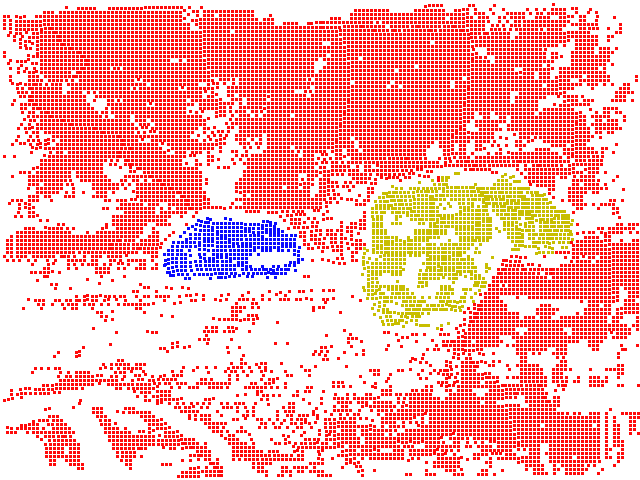
\includegraphics[width=.38\textwidth]{graphics/car-1}}%
    \only<3-4>{\\{\scriptsize image from Albert-Ludwigs-Universität,\\ 
        Lehrstuhl für Mustererkennung und Bildverarbeitung}}%
    %\only<5>{\includegraphics[width=.28\textwidth]{graphics/ml-intro/backgammon}}%
  \end{center}
\end{frame}

\begin{frame}
  \frametitle{Types of machine learning}
  \begin{definition}
    \visible<2>{Problems in which training data comprising of
      input-target pairs is available are called }\alert{supervised
      learning}\visible<2>{ problems.}
  \end{definition}
  \begin{definition}
    \visible<2>{Problems in which training data consists of input
      vectors without any target labels are called
    }\alert{unsupervised learning}\visible<2>{ problems.}
  \end{definition}
  \begin{definition}
    \visible<2>{Problems in which an agent learns actions to take in
      order to maximize a [long-term] reward are known as
    }\alert{reinforcement learning}\visible<2>{ problems.}
  \end{definition}
\end{frame}

\begin{frame}
  \frametitle{Machine Learning goals}
  Phases of a Machine Learning algorithm:
  \begin{itemize}
  \item \alert{training} a model
  \item \alert{testing} the model
  \end{itemize}
  \begin{definition}
    \visible<2>{The ability of a model to perform well on the testing
      set is called }\alert{generalization}\visible<2>{.}
  \end{definition}
\end{frame}

\begin{frame}
  \frametitle{How do we evaluate a model?}
  \begin{itemize}
  \item training set
  \item validation set
  \item test set
  \item cross-validation
  \item overfitting, underfitting
  \end{itemize}
\end{frame}


\subsection{History of research in ANN}
\label{sec:history}

\begin{frame}
  \frametitle{The neuron theory vs. the reticular theory}
  \begin{itemize}
  \item The nervous system was not properly studied until late 1800s.
  \item Camillo Golgi and \textbf{Ram\'{o}n y Cajal} $\longrightarrow$
    \emph{the neuron doctrine}.
  \end{itemize}
  \begin{center}
    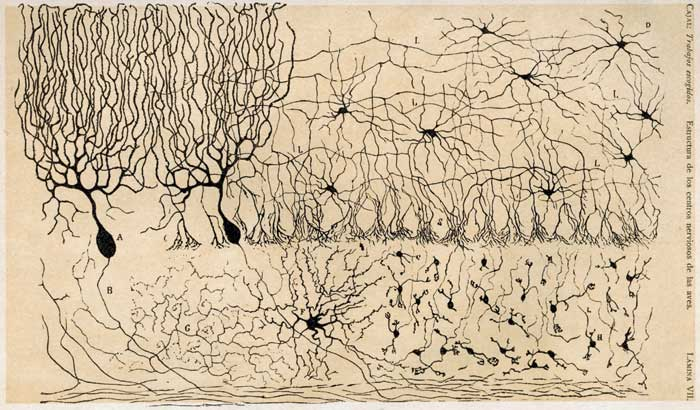
\includegraphics[height=.6\textheight]{graphics/cajal.jpg}
  \end{center}
\end{frame}

\begin{frame}
  \frametitle{McCulloch and Pitts}
  \begin{itemize}
  \item Origins of both connectionist and symbolic AI paradigms:
    \begin{itemize}
    \item \bibentry{mcculloch1943logical}
    \end{itemize}
  \item Each neuron's spike represents the truth value of a
    proposition.
  \item A neuron combines the truth values of other propositions
    (neurons) in order to compute its own.
  \end{itemize}
  \begin{center}
    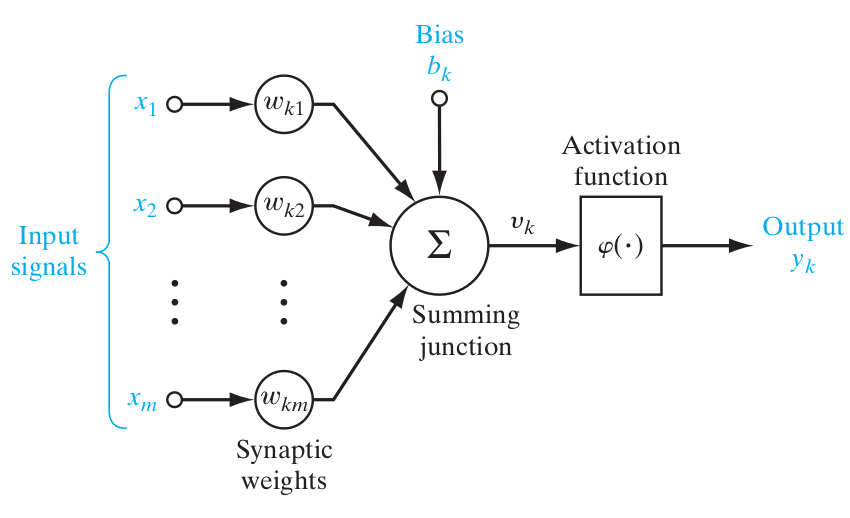
\includegraphics[height=.4\textheight]{graphics/neuron_model_haykin.png}
  \end{center}
\end{frame}

\begin{frame}
  \frametitle{Timeline}
  \begin{description}
  \item['40-'60] McCulloch and Pitts, Alan Turing, Frank Rosenblatt
  \item['69] Paper and Minsky - \emph{Perceptrons}
  \item['70 - '80] Neural Network \emph{Dark ages}
  \item['86] Rumelhart, Hinton and Williams (multi-layer perceptrons,
    error backpropagation)
  \item['00] Era of Kernel Methods (SVM, Kernel-PCA)
  \item[last years] Deep Learning
  \end{description}
\end{frame}

\subsection{Important researchers}
\label{sec:researchers}

\begin{frame}
  \frametitle{Conferences}
  There are two major annual conferences:
  \begin{itemize}
  \item Neural Information Processing Systems (\url{https://nips.cc/})
  \item International Conference on Machine Learning (\url{http://icml.cc/})
  \end{itemize}
\end{frame}

\begin{frame}
  \frametitle{Hinton's group @ University of Toronto}
  \begin{itemize}
  \item Geoffrey E. Hinton (\url{http://www.cs.toronto.edu/~hinton/})
    \begin{itemize}
    \item \url{https://www.coursera.org/course/neuralnets}
    \end{itemize}
  \item Alex Graves (\url{http://www.cs.toronto.edu/~graves/})
  \item Alex Krizhevsky (\url{http://www.cs.toronto.edu/~kriz/})
  \item Tijmen Tieleman (\url{http://www.cs.toronto.edu/~tijmen/})
  \item Ruslan Salakhutdinov (\url{http://www.cs.toronto.edu/~rsalakhu/index.html})
  \end{itemize}
  Why?
  \begin{itemize}
  \item Hinton invented most of the algorithms used today in NN.
  \item They are leading researchers in the field.
  \end{itemize}
\end{frame}

\begin{frame}
  \frametitle{Yann Lecun}
  \begin{itemize}
  \item Yann Lecun (Director of AI Research at Facebook; NY University)
    \begin{itemize}
    \item \url{http://yann.lecun.com/}
    \item \url{https://www.youtube.com/watch?v=M7smwHwdOIA}
    \end{itemize}
  \end{itemize}
  Why?
  \begin{itemize}
  \item one of the founding fathers of convolutional neural nets
  \item \emph{optimal brain damage}
  \end{itemize}
\end{frame}

\begin{frame}
  \frametitle{Yoshua Bengio}
  \begin{itemize}
  \item {\scriptsize \url{http://www.iro.umontreal.ca/~bengioy/yoshua_en/index.html}}
  \item Book still to be published:\\
    \bibentry{Goodfellow-et-al-2015-Book}
  \item Read this paper by Bengio, Hinton and Lecun: \\
    \url{http://www.nature.com/nature/journal/v521/n7553/full/nature14539.html}
  \item Read this article:
    \begin{center}
      \bibentry{Bengio:2013:DLR:2530102.2530104}
    \end{center}
  \end{itemize}
\end{frame}

\begin{frame}
  \frametitle{IDSIA}
  \begin{itemize}
  \item Jürgen Schmidhuber (\url{http://people.idsia.ch/~juergen/})
    \begin{itemize}
    \item Together with Hochreiter, inventors of LSTM \cite{hochreiter1997long}
    \item One of the pioneers of Deep Learning
      \url{http://people.idsia.ch/~juergen/deeplearning.html}
    \end{itemize}
  \item Dan Cireșan (\url{http://people.idsia.ch/~ciresan/})
  \end{itemize}
\end{frame}

\begin{frame}
  \frametitle{Google's Deep Mind}
  \begin{center}
    \url{http://deepmind.com/}
  \end{center}
  \begin{itemize}
  \item Demis Hassabis
  \item Volodymyr Mnih (\url{https://www.cs.toronto.edu/~vmnih/})
  \item Alex Graves
  \item David Silver (\url{http://www0.cs.ucl.ac.uk/staff/D.Silver/web/Home.html})
  \item Nando de Freitas
  \item ...
  \end{itemize}
  Important results:
  \begin{itemize}
  \item Deep Reinforcement Learning \cite{mnih-dqn-2015}
  \item Neural Turing Machines \cite{graves2014neural}
  \item Spatial Transformer Networks \cite{jaderberg2015spatial}
  \end{itemize}
\end{frame}

\begin{frame}
  \frametitle{Some blogs}
  \begin{itemize}
  \item Christopher Olah (Google)
    \begin{itemize}
    \item \url{http://colah.github.io/}
    \end{itemize}
  \item Andrej Karpathy (Stanford)
    \begin{itemize}
    \item \url{http://karpathy.github.io/}
    \item \url{http://cs.stanford.edu/people/karpathy/}
    \end{itemize}
  \item Yarin Gal (Cambridge)
    \begin{itemize}
    \item \url{http://mlg.eng.cam.ac.uk/yarin/blog.html}
    \end{itemize}
  \item Recent publications related to Deep Learning
    \begin{itemize}
    \item \url{http://memkite.com/deep-learning-bibliography/}
    \end{itemize}
  \end{itemize}
\end{frame}

\section{Biological Neurons and Artificial Neurons}
\label{sec:neurons}

\subsection{The Neuron}
\label{sec:neuron}

\begin{frame}
  \frametitle{The real neuron}
  \begin{figure}[h!]
    \centering
    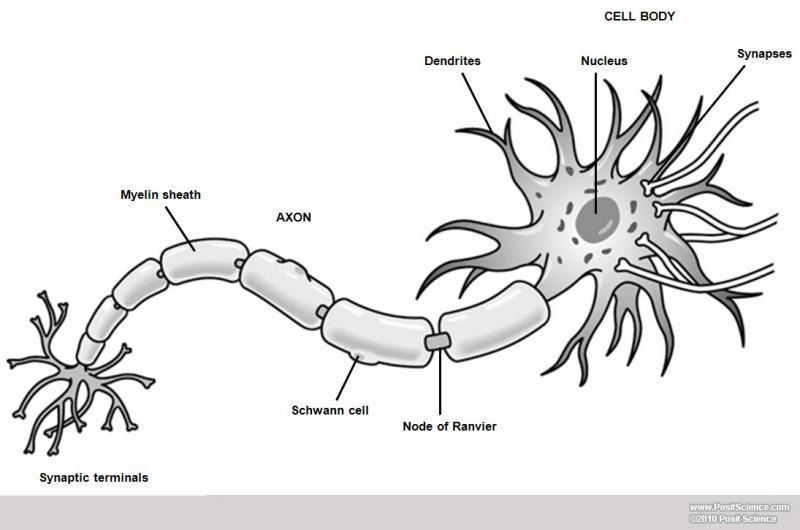
\includegraphics[height=.7\textheight]{graphics/neuron.jpg}
    \caption{A neuron from the CNS}
    \label{fig:realneuron}
  \end{figure}
\end{frame}

\begin{frame}
  \frametitle{The McCulloch-Pitts neuron}
  \begin{figure}[h!]
    \centering
    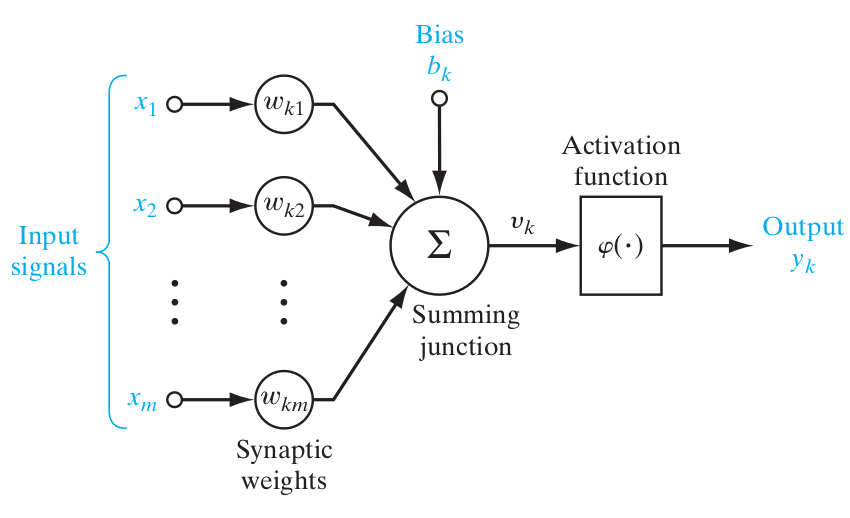
\includegraphics[height=.7\textheight]{graphics/neuron_model_haykin.png}
    \caption{The McCulloch-Pitts neuron model (taken from \cite{haykin2009neural})}
    \label{fig:realneuron}
  \end{figure}
\end{frame}


\begin{frame}
  \frametitle{Neuron Models}
  \begin{itemize}
  \item when building ANNs we do not consider
    the full complexity of real biological neurons
  \item models exclude details that are not useful
  \item on simplified models we can apply mathematics
  \end{itemize}
\end{frame}

\subsection{Neuronal models}
\label{sec:neuronal_models}

\begin{frame}
  \frametitle{Elements of the neural model}
  The basic elements of the neural model:
  \begin{description}
  \item[connecting links] - each characterized by a synaptic weight
  \item[adder] - a function that sums the inputs (\emph{linear combiner)}
  \item[activation function] - limits the amplitude of the neuron
  \end{description}
\end{frame}

\begin{frame}
  \frametitle{Linear neurons}
  \begin{definition}
    \alert{Linear neurons}:
    \begin{equation}
      \label{eq:linear-neuron}
      y_k = b_k + \displaystyle\sum_{i}x_i\cdot w_{ki}
    \end{equation}
    \begin{description}
    \item[$y_k$] - output of the neuron
    \item[$b_k$] - bias
    \item[$i$] - index over input synapses
    \item[$x_i$] - $i^{th}$ input
    \item[$w_{ki}$] - weight for connection between neuron $k$ and input $i$
    \end{description}
  \end{definition}
\end{frame}

\begin{frame}
  \frametitle{Linear neurons}
  \begin{figure}[h!]
    \centering
    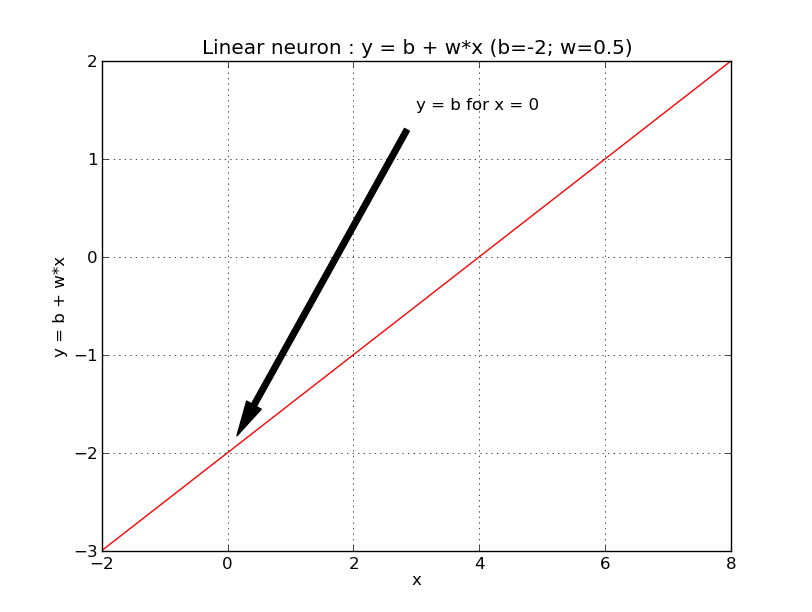
\includegraphics[width=.7\textwidth]{graphics/linear_neuron.png}
    \caption{Linear neuron $y = b + w \cdot x$ for $w = 0.5,b=-2$}
    \label{fig:linearneuron}
  \end{figure}
\end{frame}

\begin{frame}
  \frametitle{Binary Threshold Neurons}
  \begin{definition}
    \alert{Binary threshold neurons (McCulloch and Pitts, 1943)}:
    \begin{equation}
      \label{eq:binary-threshold-neuron-1}
      z_k = b_k + \displaystyle\sum_{i}x_i\cdot w_{ki}
    \end{equation}
    \begin{equation}
      \label{eq:binary-threshold-neuron-2}
      y_k = \begin{cases} 0 & \text{if } z_k < 0 \\ 1 & \text{if } z_k \ge 0 \end{cases}
    \end{equation}
    \begin{description}
    \item[$y_k$] - output of the neuron
    \item[$b_k$] - bias
    \item[$x_i$] - $i^{th}$ input
    \item[$w_{ki}$] - weight for connection between neuron $k$ and input $i$
    \item[$z_k$] - induced local field
    \end{description}
  \end{definition}
\end{frame}

\begin{frame}
  \frametitle{Binary Threshold Neuron}
  \begin{figure}[h!]
    \centering
    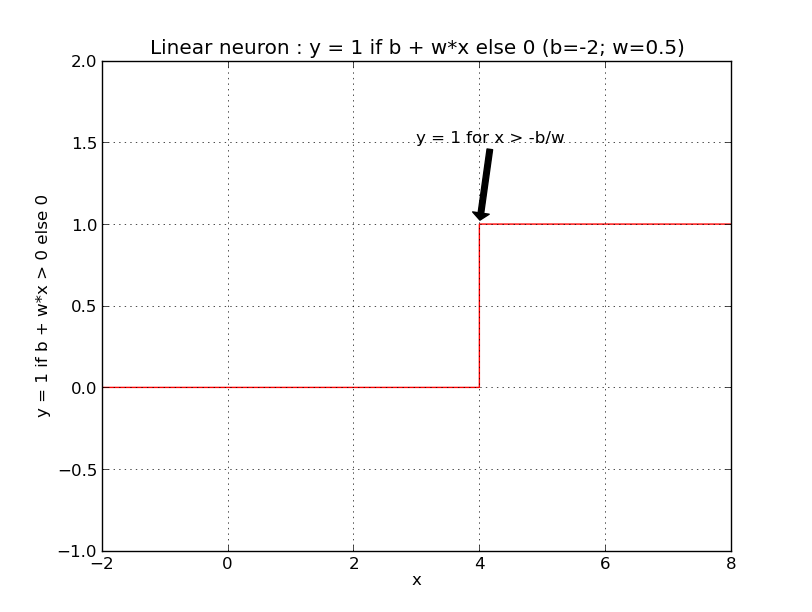
\includegraphics[height = .7\textheight]{graphics/binary_threshold_neuron.png}
    \caption{Binary Threshold Neuron}
  \end{figure}
\end{frame}

\begin{frame}
  \frametitle{Rectified Linear Neurons}
  \begin{definition}
    \alert{Rectified linear neurons}:
    \begin{equation}
      \label{eq:rectified-linear-neuron-1}
      z_k = b_k + \displaystyle\sum_{i}x_i\cdot w_{ki}
    \end{equation}
    \begin{equation}
      \label{eq:rectified-linear-neuron-2}
      y_k = \begin{cases} z_k & \text{if } z_k \ge 0 \\ 0 & \text{if } z_k < 0 \end{cases}
    \end{equation}
    \begin{description}
    \item[$y_k$] - output of the neuron
    \item[$b_k$] - bias
    \item[$x_i$] - $i^{th}$ input
    \item[$w_{ki}$] - weight for connection between neuron $k$ and input $i$
    \item[$z_k$] - induced local field
    \end{description}
  \end{definition}
\end{frame}

\begin{frame}
  \frametitle{Rectified Linear Neuron}
  \begin{figure}[h!]
    \centering
    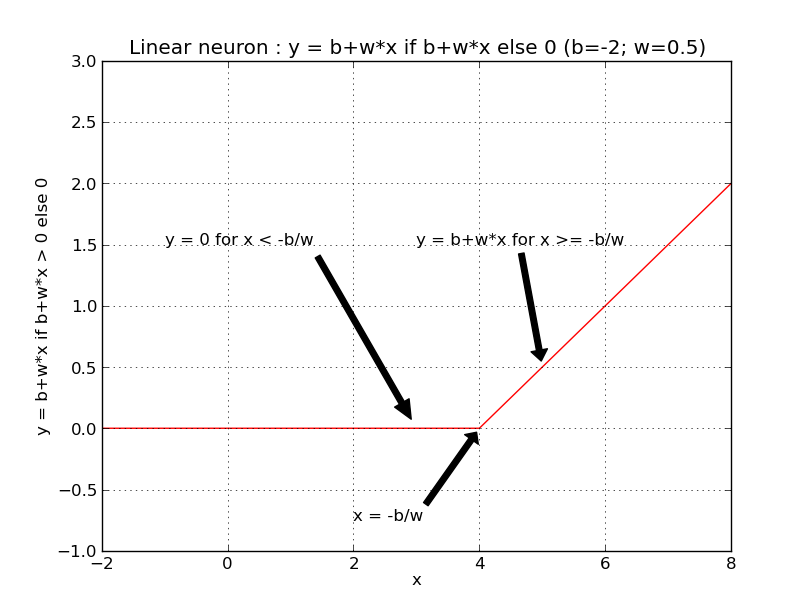
\includegraphics[height = .7\textheight]{graphics/rectified_linear_neuron.png}
    \caption{Rectified Linear Neuron}
  \end{figure}
\end{frame}

\begin{frame}
  \frametitle{Sigmoid neurons I}
  \begin{itemize}
  \item the binary threshold neuron activation function is not
    differentiable
  \item smooth, continuous functions that approximate the Heaviside
    step function would be nice
  \item easy to compute derivatives would be great too
  \end{itemize}
\end{frame}

\begin{frame}
  \frametitle{Sigmoid neurons II}
  \begin{definition}
    \begin{equation}
      \label{eq:logistic-neuron-1}
      z_k = b_k + \displaystyle\sum_{i}x_i\cdot w_{ki}
    \end{equation}
    The logistic function for activation:
    \begin{equation}
      \label{eq:logistic-neuron-2}
      y_k = \frac{1}{1 + e^{\alpha \cdot z_k}}
    \end{equation}
  \end{definition}
  \begin{itemize}
  \item Here is the nice derivative:
    \begin{equation}
      \label{eq:logistic-derivative}
      \frac{d}{dx}f(x) = f(x) \cdot (1 - f(x))
    \end{equation}
  \end{itemize}
\end{frame}

\begin{frame}
  \frametitle{Logistic function I}
  \begin{figure}[h!]
    \centering
    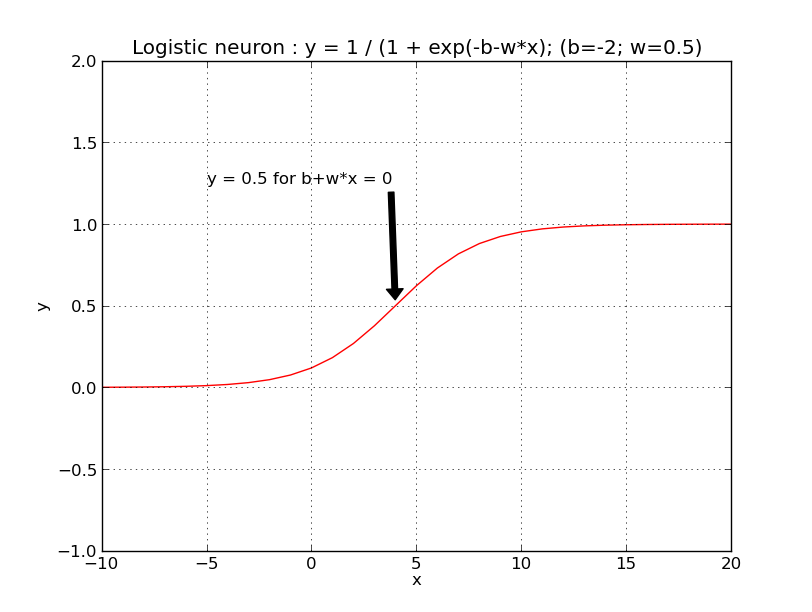
\includegraphics[height = .7\textheight]{graphics/logistic_neuron.png}
    \caption{Logistic function}
  \end{figure}
\end{frame}

\begin{frame}
  \frametitle{Logistic function II}
  \begin{figure}[h!]
    \centering
    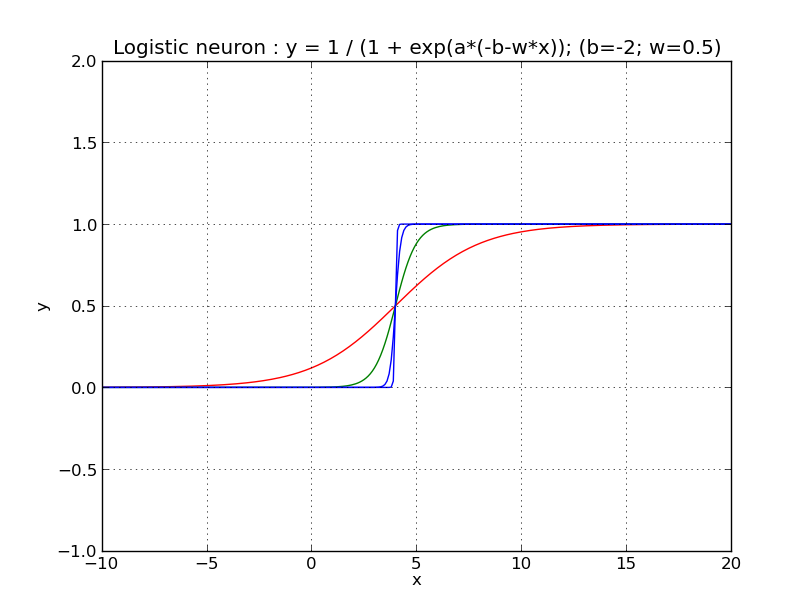
\includegraphics[height = .7\textheight]{graphics/logistic-neuron-2.png}
    \caption{Logistic function for different values for $\alpha$}
  \end{figure}
\end{frame}

\begin{frame}
  \frametitle{Hyperbolic tangent}
  \begin{definition}
    \begin{equation}
      \label{eq:hyperbolic-neuron-1}
      z_k = b_k + \displaystyle\sum_{i}x_i\cdot w_{ki}
    \end{equation}
    The logistic function for activation:
    \begin{equation}
      \label{eq:hyperbolic-neuron-2}
      y_k = \frac{e^{z_k}-e^{-z_k}}{e^{z_k}+e^{-z_k}}
    \end{equation}
  \end{definition}
  \begin{center}
    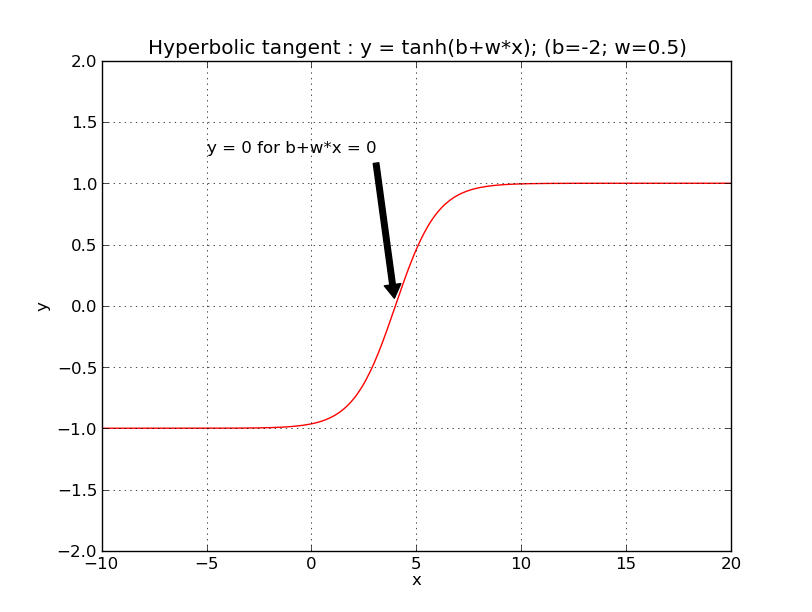
\includegraphics[height = .4\textheight]{graphics/hyperbolic_neuron.png}
  \end{center}
\end{frame}


\begin{frame}
  \frametitle{Stochastic neurons}
  \begin{itemize}
  \item use the same logistic activation function, but as a
    probability of firing
  \end{itemize}
  \begin{definition}
    Stochastic binary neurons:
    \begin{equation}
      \label{eq:stochastic-neuron-1}
      z_k = b_k + \displaystyle\sum_{i}x_i\cdot w_{ki}
    \end{equation}
    The probability of being active:
    \begin{equation}
      \label{eq:logistic-neuron-2}
      p(y_k = 1) = \frac{1}{1 + e^{z_k}}
    \end{equation}
  \end{definition}
\end{frame}

\section{Torch}
\label{sec:torch}

\subsection{Why Torch?}
\label{sec:why_torch}

\begin{frame}
  \frametitle{What is Torch?}
  \begin{itemize}
  \item Torch7 (\url{http://torch.ch/})
  \item scientific computing framework for machine learning
  \item uses a fast scripting language: Lua
  \end{itemize}
\end{frame}

\begin{frame}
  \frametitle{Why Torch?}
  \begin{itemize}
  \item really fast neural networks and optimization libraries
  \item large list of community-driven packages
  \item automatic parallelization over CPUs and GPUs
  \item contributors:
    \begin{itemize}
    \item researchers @ Deep Mind
    \item researchers @ Facebook
      \url{https://research.facebook.com/blog/879898285375829/fair-open-sources-deep-learning-modules-for-torch/}
    \item Twitter, NVIDIA, AMD, etc.
    \end{itemize}
    \vfill
  \item Read this comparison between various machine learning platforms: {\scriptsize \url{https://github.com/zer0n/deepframeworks/blob/master/README.md}}
  \end{itemize}
\end{frame}

\subsection{Short Introduction to Lua}
\label{sec:intro_to_torch}

\begin{frame}
  \frametitle{Introduction to Lua}
  \begin{center}
    The following slides follow the Lua tutorial from here:
    \url{http://tylerneylon.com/a/learn-lua/}. \\
    \vfill
    Read the full tutorial!
  \end{center}
\end{frame}

\begin{frame}[fragile]
  \frametitle{Comments and Variables in Lua}
  \begin{minted}[mathescape, linenos, numbersep=5pt, gobble=2,
    frame=lines, framesep=2mm]{lua}
  -- Two dashes start a one-line comment.

  --[[
     Adding two ['s and ]'s makes it a
     multi-line comment.
  --]]

  x = 23
  \end{minted}
  \begin{center}
    \begin{tiny}
      source: \url{http://tylerneylon.com/a/learn-lua/}.
    \end{tiny}
  \end{center}
\end{frame}

\begin{frame}[fragile]
  \frametitle{Data Types in Lua; Garbage Collection}
  \begin{minted}[mathescape, linenos, numbersep=5pt, gobble=2,
    frame=lines, framesep=2mm]{lua}
  num = 42  -- All numbers are doubles.
  -- Don't freak out, 64-bit doubles have 52 bits for
  -- storing exact int values; machine precision is
  -- not a problem for ints that need < 52 bits.

  s = 'walternate'  -- Immutable strings like Python.
  t = "double-quotes are also fine"
  u = [[ Double brackets
         start and end
         multi-line strings.]]
  t = nil  -- Undefines t; Lua has garbage collection.
  \end{minted}
  \begin{center}
    \begin{tiny}
      source: \url{http://tylerneylon.com/a/learn-lua/}.
    \end{tiny}
  \end{center}
\end{frame}

\begin{frame}[fragile]
  \frametitle{Flow Control (I)}
  \begin{minted}[mathescape, linenos, numbersep=5pt, gobble=2,
    frame=lines, framesep=2mm]{lua}
  -- Blocks are denoted with keywords like do/end:
  while num < 50 do
    num = num + 1  -- No ++ or += type operators.
  end
  \end{minted}
  \begin{center}
    \begin{tiny}
      source: \url{http://tylerneylon.com/a/learn-lua/}.
    \end{tiny}
  \end{center}
\end{frame}

\begin{frame}[fragile]
  \frametitle{Flow Control (II)}
  \begin{minted}[mathescape, linenos, numbersep=5pt, gobble=2,
    frame=lines, framesep=2mm]{lua}
  -- If clauses:
  if num > 40 then
    print('over 40')
  elseif s ~= 'walternate' then  -- ~= is not equals.
    -- Equality check is == like Python; ok for strs.
    io.write('not over 40\n')  -- Defaults to stdout.
  else
    -- Variables are global by default.
    thisIsGlobal = 5  -- Camel case is common.
    -- How to make a variable local:
    local line = io.read()  -- Reads next stdin line.
    -- String concatenation uses the .. operator:
    print('Winter is coming, ' .. line)
  end
  \end{minted}
  \begin{center}
    \begin{tiny}
      source: \url{http://tylerneylon.com/a/learn-lua/}.
    \end{tiny}
  \end{center}
\end{frame}

\begin{frame}[fragile]
  \frametitle{Falsy values}
  \begin{minted}[mathescape, linenos, numbersep=5pt, gobble=2,
    frame=lines, framesep=2mm]{lua}
  -- Undefined variables return nil.
  -- This is not an error:
  foo = anUnknownVariable  -- Now foo = nil.

  aBoolValue = false

  -- Only nil and false are falsy; 0 and '' are true!
  if not aBoolValue then print('twas false') end

  -- 'or' and 'and' are short-circuited.
  ans = aBoolValue and 'yes' or 'no'  --> 'no'
  \end{minted}
  \begin{center}
    \begin{tiny}
      source: \url{http://tylerneylon.com/a/learn-lua/}.
    \end{tiny}
  \end{center}
\end{frame}

\begin{frame}[fragile]
  \frametitle{Falsy values}
  \begin{minted}[mathescape, linenos, numbersep=5pt, gobble=2,
    frame=lines, framesep=2mm]{lua}
  karlSum = 0
  for i = 1, 100 do  -- The range includes both ends.
    karlSum = karlSum + i
  end
  -- Use "100, 1, -1" as the range to count down:
  fredSum = 0
  for j = 100, 1, -1 do fredSum = fredSum + j end
  \end{minted}
  \begin{center}
    \begin{tiny}
      source: \url{http://tylerneylon.com/a/learn-lua/}.
    \end{tiny}
  \end{center}
\end{frame}


\begin{frame}[fragile]
  \frametitle{Another loop construct}
  \begin{minted}[mathescape, linenos, numbersep=5pt, gobble=2,
    frame=lines, framesep=2mm]{lua}
  repeat
    print('the way of the future')
    num = num - 1
  until num == 0
  \end{minted}
  \vfill
  \begin{center}
    \begin{tiny}
      source: \url{http://tylerneylon.com/a/learn-lua/}.
    \end{tiny}
  \end{center}
\end{frame}


\begin{frame}[fragile]
  \frametitle{Functions}
  \begin{minted}[mathescape, linenos, numbersep=5pt, gobble=2,
    frame=lines, framesep=2mm]{lua}
  function fib(n)
    if n < 2 then return 1 end
    return fib(n - 2) + fib(n - 1)
  end
  \end{minted}
  \vfill
  \begin{center}
    \begin{tiny}
      source: \url{http://tylerneylon.com/a/learn-lua/}.
    \end{tiny}
  \end{center}
\end{frame}


\begin{frame}[fragile]
  \frametitle{Anonymous functions}
  \begin{minted}[mathescape, linenos, numbersep=5pt, gobble=2,
    frame=lines, framesep=2mm]{lua}
  -- Closures and anonymous functions are ok:
  function adder(x)
    -- The returned function is created when adder is
    -- called, and remembers the value of x:
    return function (y) return x + y end
  end
  a1 = adder(9)
  a2 = adder(36)
  print(a1(16))  --> 25
  print(a2(64))  --> 100
  \end{minted}
  \vfill
  \begin{center}
    \begin{tiny}
      source: \url{http://tylerneylon.com/a/learn-lua/}.
    \end{tiny}
  \end{center}
\end{frame}


\begin{frame}[fragile]
  \frametitle{Functions' senders and receivers}
  \begin{minted}[mathescape, linenos, numbersep=5pt, gobble=2,
    frame=lines, framesep=2mm]{lua}
  -- Returns, func calls, and assignments all work
  -- with lists that may be mismatched in length.
  -- Unmatched receivers are nil;
  -- unmatched senders are discarded.

  x, y, z = 1, 2, 3, 4
  -- Now x = 1, y = 2, z = 3, and 4 is thrown away.

  function bar(a, b, c)
    print(a, b, c)
    return 4, 8, 15, 16, 23, 42
  end
  x, y = bar('zaphod')  --> prints "zaphod  nil nil"
  -- Now x = 4, y = 8, values 15..42 are discarded.
  \end{minted}
  \vfill
  \begin{center}
    \begin{tiny}
      source: \url{http://tylerneylon.com/a/learn-lua/}.
    \end{tiny}
  \end{center}
\end{frame}


\begin{frame}[fragile]
  \frametitle{Functions are first class values}
  \begin{minted}[mathescape, linenos, numbersep=5pt, gobble=2,
    frame=lines, framesep=2mm]{lua}
  -- Functions are first-class, may be local/global.
  -- These are the same:
  function f(x) return x * x end
  f = function (x) return x * x end

  -- And so are these:
  local function g(x) return math.sin(x) end
  local g; g  = function (x) return math.sin(x) end
  -- the 'local g' decl makes g-self-references ok.
  \end{minted}
  \vfill
  \begin{center}
    \begin{tiny}
      source: \url{http://tylerneylon.com/a/learn-lua/}.
    \end{tiny}
  \end{center}
\end{frame}


\begin{frame}[fragile]
  \frametitle{Another loop construct}
  \begin{minted}[mathescape, linenos, numbersep=5pt, gobble=2,
    frame=lines, framesep=2mm]{lua}
  -- Tables = Lua's only compound data structure;
  --          they are associative arrays.
  -- Similar to php arrays or js objects, they are
  -- hash-lookup dicts that can also be used as lists.

  -- Using tables as dictionaries / maps:

  -- Dict literals have string keys by default:
  t = {key1 = 'value1', key2 = false}
  \end{minted}
  \vfill
  \begin{center}
    \begin{tiny}
      source: \url{http://tylerneylon.com/a/learn-lua/}.
    \end{tiny}
  \end{center}
\end{frame}


\begin{frame}[fragile]
  \frametitle{Another loop construct}
  \begin{minted}[mathescape, linenos, numbersep=5pt, gobble=2,
    frame=lines, framesep=2mm]{lua}
  -- Dict literals have string keys by default:
  t = {key1 = 'value1', key2 = false}

  -- String keys can use js-like dot notation:
  print(t.key1)  -- Prints 'value1'.
  t.newKey = {}  -- Adds a new key/value pair.
  t.key2 = nil   -- Removes key2 from the table.

  -- Literal notation for any (non-nil) value as key:
  u = {['@!#'] = 'qbert', [{}] = 1729, [6.28] = 'tau'}
  print(u[6.28])  -- prints "tau"
  \end{minted}
  \vfill
  \begin{center}
    \begin{tiny}
      source: \url{http://tylerneylon.com/a/learn-lua/}.
    \end{tiny}
  \end{center}
\end{frame}


\begin{frame}[fragile]
  \frametitle{Another loop construct}
  \begin{minted}[mathescape, linenos, numbersep=5pt, gobble=2,
    frame=lines, framesep=2mm]{lua}
  -- Key matching is basically by value for numbers
  -- and strings, but by identity for tables.
  a = u['@!#']  -- Now a = 'qbert'.
  b = u[{}]     -- We might expect 1729, but it's nil:
  -- b = nil since the lookup fails. It fails
  -- because the key we used is not the same object
  -- as the one used to store the original value. So
  -- strings & numbers are more portable keys.
  \end{minted}
  \vfill
  \begin{center}
    \begin{tiny}
      source: \url{http://tylerneylon.com/a/learn-lua/}.
    \end{tiny}
  \end{center}
\end{frame}

\begin{frame}[fragile]
  \frametitle{Another loop construct}
  \begin{minted}[mathescape, linenos, numbersep=5pt, gobble=2,
    frame=lines, framesep=2mm]{lua}
  -- A one-table-param function call needs no parens:
  function h(x) print(x.key1) end
  h{key1 = 'Sonmi~451'}  -- Prints 'Sonmi~451'.

  for key, val in pairs(u) do  -- Table iteration.
    print(key, val)
  end
  \end{minted}
  \vfill
  \begin{center}
    \begin{tiny}
      source: \url{http://tylerneylon.com/a/learn-lua/}.
    \end{tiny}
  \end{center}
\end{frame}


\begin{frame}[fragile]
  \frametitle{Another loop construct}
  \begin{minted}[mathescape, linenos, numbersep=5pt, gobble=2,
    frame=lines, framesep=2mm]{lua}
  -- _G is a special table of all globals.
  print(_G['_G'] == _G)  -- Prints 'true'.
  \end{minted}
  \vfill
  \begin{center}
    \begin{tiny}
      source: \url{http://tylerneylon.com/a/learn-lua/}.
    \end{tiny}
  \end{center}
\end{frame}


\begin{frame}[fragile]
  \frametitle{Another loop construct}
  \begin{minted}[mathescape, linenos, numbersep=5pt, gobble=2,
    frame=lines, framesep=2mm]{lua}
  -- Using tables as lists / arrays:

  -- List literals implicitly set up int keys:
  v = {'value1', 'value2', 1.21, 'gigawatts'}
  for i = 1, #v do  -- #v is the size of v for lists.
    print(v[i])  -- Indices start at 1 !! SO CRAZY!
  end
  -- A 'list' is not a real type. v is just a table
  -- with consecutive integer keys, treated as a list.
  \end{minted}
  \vfill
  \begin{center}
    \begin{tiny}
      source: \url{http://tylerneylon.com/a/learn-lua/}.
    \end{tiny}
  \end{center}
\end{frame}

\appendix

\section{For the exam}
\label{sec:readings}

\begin{frame}
  \frametitle{What to read}
  Read ...
  \begin{itemize}
  \item ... the \emph{Introduction} chapter from \cite{haykin2009neural}
  \end{itemize}
\end{frame}

\begin{frame}
  \frametitle{Topics for the exam}
  \begin{itemize}
  \item For the exam you should be able to:
    \begin{itemize}
    \item ... define basic machine learning concepts (e.g. regression,
      classification, cross-validation);
    \item ... give a general description of artificial neural networks
      (why is it worth studying them, how do they resemble biological
      neural networks);
    \item ... know the usual activation functions used in artificial
      neural networks.
    \end{itemize}
  \end{itemize}
\end{frame}

\section{References}%
\label{sec:references}%

\begin{frame}[allowframebreaks]{References}%
  \def\newblock{}%
  \bibliographystyle{amsalpha}%
  \bibliography{ann}%
\end{frame}%


\end{document}